\documentclass[11pt, oneside]{article} 
\usepackage{geometry}
\geometry{letterpaper} 
\usepackage{graphicx}
	
\usepackage{amssymb}
\usepackage{amsmath}
\usepackage{parskip}
\usepackage{color}
\usepackage{hyperref}

\graphicspath{{/Users/telliott_admin/Tex/png/}}
% \begin{center} 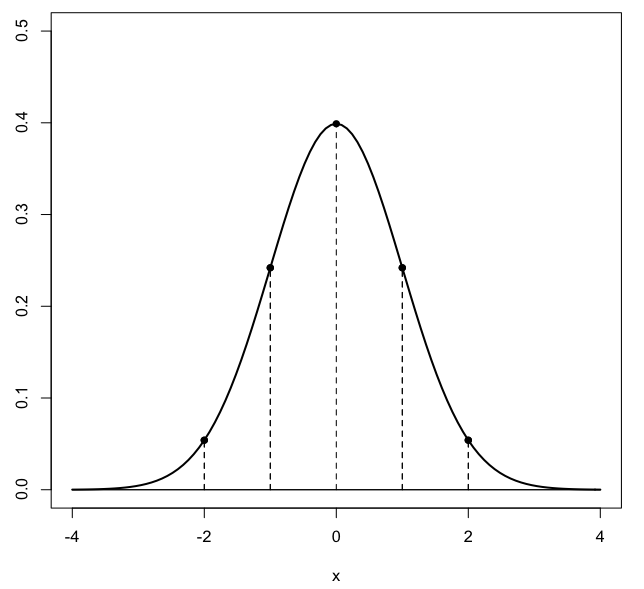
\includegraphics [scale=0.4] {gauss3.png} \end{center}

\title{Tablet of integrals}
\date{}

\begin{document}
\maketitle
\Large

I thought we could work on the derivations of some of the integrals shown in standard tables.  

Here is what I have so far.  Each one of the following will come in three versions [ A:  ($x^2 + 1$), B:  ($x^2 - 1$), C:  ($1 - x^2$) ].  Let's group them as follows:

\begin{equation} \int \frac{1}{\sqrt{x^2 + 1}} \ dx \end{equation}
\begin{equation} \int \sqrt{x^2 + 1} \ dx \end{equation}
\begin{equation} \int \frac{1}{x^2 + 1} \ dx \end{equation}
\begin{equation} \int \frac{x^2}{\sqrt{x^2 +1}} \ dx \end{equation}
\begin{equation} \int \frac{1}{x\sqrt{x^2 + 1}} \ dx \end{equation}
\begin{equation} \int \frac{1}{x^2 \sqrt{x^2 + 1}} \ dx \end{equation}

In every case, we can also deal with a similar integral containing $x^2 + a^2$ (i.e. $a^2$ substituted for $1$).  This is done either by factoring the $a$ part out or by setting up a trig substitution a little differently.  For the most part, we'll just keep it simple, but we'll look at the effect of having $a^2$ in place of $1$  for a few examples as shown below.  

Let's see how far we get.

\section*{1A $\int 1/\sqrt{x^2 + 1} \ dx$ }

This one is fairly simple, a "trig substitution".  Since we have $\sqrt{x^2 + 1}$, this suggests a right triangle with two sides $x$ and $1$, and hypotenuse $\sqrt{x^2 + 1}$.  We will have a right triangle with angle $t$, and then imagine that we have opposite and adjacent sides:

\[ \text{opp} = x, \ \ \text{adj} = 1 \]

and hypotenuse

\[ \ \ \text{hyp} = \sqrt{x^2 + 1}   \]

and, in terms of the trig functions, we obtain:

\[ x = \tan t, \ \ dx = \sec^2 t  \ dt, \ \ 1/\sqrt{x^2 + 1} = \cos t \]

This gives:

\[ = \int \cos t \sec^2 t \ dt \]
\[ = \int \sec t \ dt \]
\[ = \ln | \ \sec t + \tan t \ | + c \]

Substitute back with $x$ and finally we have, in summary:

\[ \int \frac{1}{\sqrt{x^2 + 1}} \ dx = \ln | \ x + \sqrt{x^2 + 1} \  | + C \]

\subsection*{check}

\[ \frac{d}{dx} \ln | \ x + \sqrt{x^2 + 1}  \ | \]
\[ = \frac{1}{x + \sqrt{x^2 + 1} } ( 1 + \frac{x}{\sqrt{x^2 + 1}}) \]
\[ = \frac{1}{x + \sqrt{x^2 + 1} } ( \frac{\sqrt{x^2 + 1} + x }{\sqrt{x^2 + 1}} ) \]
\[ = \frac{1}{\sqrt{x^2 + 1}} \]

\subsection*{dealing with $a^2$}

Let's think about how we'd have to change things for $x^2 + a^2$.  One approach is to change the trig functions.  Change the side with length $1$ to have length $a$, then with hypotenuse $\sqrt{x^2 + a^2}$, we have

\[ \frac{x}{a} = \tan t, \ \  dx = a \sec^2 t  \ dt, \ \ a/\sqrt{x^2 + a^2} = \cos t \]

\[ \int \frac{1}{\sqrt{x^2 + a^2}} \ dx = \int \frac{1}{a} \cos t \ a \sec^2 t \ dt = \int \sec t \ dt \]

We have the same integral and obtain almost the same answer as before

\[ = \ln | \ \sec t + \tan t \ | + c \]
\[ = \ln | \ \frac{1}{a} ( \sqrt{x^2 + a^2}  + x) \ | \ + C \]

\subsection*{check}

We should check this result.

\[ \frac{d}{dx} \ln \ | \ \frac{1}{a} ( \sqrt{x^2 + a^2}  + x) \ | \    \]

\[ =  \frac{a}{x + \sqrt{x^2 + a^2}}  \cdot \frac{1}{a} (\frac{x}{\sqrt{x^2 + a^2}} + 1 ) \]

\[ = \frac{1}{x + \sqrt{x^2 + a^2}}  \cdot \frac{x + \sqrt{x^2 + a^2} }{\sqrt{x^2 + a^2}}  = \frac{1}{\sqrt{x^2 + a^2}} \]

\subsection*{factoring method}

A second approach is to factor out the $a$, obtaining

\[ \int \frac{1}{ \sqrt{x^2 + a^2}} \ dx =  \frac{1}{a}  \int  \frac{1}{ \sqrt{(x/a)^2 + 1}}  \ dx \]

I think of this as multiplying "on the top and on the bottom" by $1/a$, with the factor out in front being the multiplication on the top.  Now, substitute

\[ u = x/a, \ \ a \ du = dx \]

\[ \frac{1}{a}  \int  \frac{1}{ \sqrt{(x/a)^2 + 1}}  \ dx = \int \frac{1}{ \sqrt{u^2 + 1}}\ du \]

\[ = \ln | \ \sqrt{u^2 + 1} + u \ | + C \]
\[ = \ln \ | \ \sqrt{(x/a)^2 + 1} + x/a \ | + C \]
\[ = \ln \ | \ \frac{1}{a} \sqrt{x^2 + a^2} + \frac{1}{a} x \ | + C \]
\[ = \ln | \ \frac{1}{a} ( \sqrt{x^2 + a^2}  + x) \ | \ + C \]

as we had before.

\subsection*{inverse hyperbolic sine}

There is actually \emph{another} version of the answer to this problem.  It involves the hyperbolic sine, which is defined as follows 

\[ \sinh x = \frac{e^x - e^{-x}}{2} \]
\[ \cosh x = \frac{e^x + e^{-x}}{2} \]

The answer is 

\[ \int \frac{1}{ \sqrt{x^2 + a^2}} \ dx = \sinh^{-1} \frac{x}{a} \]

Proof.  Represent the value of the integral as $z$, then

\[ z = \sinh^{-1} \frac{x}{a} \]
\[ \frac{x}{a} = \sinh z \]
\[ \frac{x}{a} = \frac{1}{2} (e^z - e^{-z}) \]

Solve for $z$.  Let $u = e^z$ so we have

\[ \frac{2x}{a} = u - \frac{1}{u} \]
\[ au^2 - 2xu - a = 0 \]

The roots are

\[ u = \frac{2x  \pm \sqrt{4x^2 + 4a^2}}{2a} \]
\[ u = \frac{x  \pm \sqrt{x^2 + a^2}}{a} \]

For real $z$, $e^z > 0$ so we need the positive root

\[ u = \frac{x  + \sqrt{x^2 + a^2}}{a} \]

Go back to $z$

\[ e^z = \frac{x  + \sqrt{x^2 + a^2}}{a} \]
\[ z = \ln |x  + \sqrt{x^2 + a^2}| - \ln a \]

\section*{1B $\int 1/\sqrt{x^2 - 1} \ dx$}

This one seems a bit easier.  Again, do a trig substitution.  

\[ \text{hyp} = x, \ \ \text{adj} = 1, \ \ \text{opp} = \sqrt{x^2 - 1}   \]

Now, $x = \sec t$, $dx = \sec t \tan t \ dt$, and $\sqrt{x^2 - 1} = \tan t$

\[ = \int \frac{1}{\tan t} \sec t \tan t \ dt \]
\[ = \int \sec t \ dt \]

The same as for \# 1A except for the minus sign under the square root.

\[ = \ln | \sec t + \tan t | + c = \ln | x + \sqrt{x^2 - 1} | + C \]

\subsection*{check}

\[ \frac{1}{x + \sqrt{x^2-1}} \ (1 + \frac{x}{\sqrt{x^2-1}} ) \]
\[ = \frac{1}{x + \sqrt{x^2-1}} \ (\frac{\sqrt{x^2-1} + x}{\sqrt{x^2-1}}  ) = \frac{1}{\sqrt{x^2-1}}\]

\subsection*{dealing with $a^2$}

\[ \int \frac{1}{\sqrt{x^2 - a^2}} \ dx \]

Our substitution is now

\[ \text{hyp} = x, \ \ \text{adj} = a, \ \ \text{opp} = \sqrt{x^2 - a^2}   \]

with $x = a \sec t$, $dx = a \sec t \tan t \ dt$, and $\sqrt{x^2 - a^2} = a \tan t$.  Then the integral becomes 

\[ \int \frac{1}{a \tan t} \ a \sec t \tan t \ dt \]

The integral comes out just as before:   $\ln \ | \ \sec t + \tan t \ |$, but the substitution back to $x$ gives an extra factor of $1/a$ for both terms:

\[ = \ln \ | \ \frac{x}{a} + \frac{1}{a} \sqrt{x^2 - a^2}  \ | \]

These two results (A and B) are usually combined and written

\[ \int \frac{1}{ \sqrt{x^2 \pm a^2}} \ dx = \ln | \ \frac{1}{a} \sqrt{x^2 \pm a^2}  + \frac{1}{a} x \ | \ + C \]

\section*{1C $\int 1/\sqrt{1 - x^2} \ dx$}

This one is just $\sin^{-1} x$.  We get that by

\[ \text{opp} = x, \ \ \text{hyp} = 1, \ \ \text{adj} = \sqrt{1 - x^2}   \]

So 

\[ x = \sin t \]
\[ t = \sin^{-1} x \]
\[ \frac{dx}{dt} = \cos t = \sqrt{1-x^2}\]
\[ \frac{dt}{dx} = \frac{1}{\cos t} = \frac{1}{\sqrt{1-x^2}} \]

The answer is

\[ \int \frac{1}{\sqrt{1 - x^2}} = \sin^{-1} x \]

\subsection*{dealing with $a^2$}

It's easy to see that we will have

\[ \int \frac{1}{\sqrt{a^2 - x^2}} = \sin^{-1} \frac{x}{a} \]

\begin{center} \line(1,0){250} \end{center}

\section*{2A $\int \sqrt{x^2 + 1} \ dx$}

Multiply top and bottom by what's on the top

\[ = \int \frac{x^2 + 1}{\sqrt{x^2 + 1}} \ dx \]
\[ =  \int \frac{x^2}{\sqrt{x^2 + 1}} + \frac{1}{\sqrt{x^2 + 1}} \ dx \]

The term on the right is \# 1A from above.  The answer is:

\[  \ln |\sqrt{x^2+1} + x| + C \]

Now for the term on the left.  That is actually \# 4A.  The answer (still with an integral in it) is:

\[ \int \frac{x^2}{\sqrt{x^2 + 1}} \ dx = x \sqrt{x^2 + 1} - \int \sqrt{x^2 + 1} \ dx + C \]

We've come full circle.  Appearing in the answer is minus the same integral that we started with.  It's OK.  We assemble everything, grouping the two identical terms on the left, divide by 2, and obtain:

\[ \int \sqrt{x^2 + 1} \ dx = \frac{1}{2} \ x \sqrt{x^2 + 1} + \frac{1}{2} \ln |\ \sqrt{x^2 + 1} + x \ | + C \] 

\subsection*{check}

Leave the factor of $1/2$ aside for the moment.  The derivative of the first term is

\[ \sqrt{x^2 + 1} + \frac{x^2}{\sqrt{x^2 + 1}} \]

We checked the second term above in \# 1A, it is just

\[ \frac{1}{\sqrt{x^2 + 1}} \]

So now we have 

\[ \sqrt{x^2 + 1} + \frac{x^2}{\sqrt{x^2 + 1}} +  \frac{1}{\sqrt{x^2 + 1}} \]
\[ = \frac{x^2 + 1}{\sqrt{x^2 + 1}} + \frac{x^2}{\sqrt{x^2 + 1}} +  \frac{1}{\sqrt{x^2 + 1}} \]
\[ = \frac{2(x^2 + 1)}{\sqrt{x^2 + 1}} \]

Remember the factor of $1/2$, and simplify

\[ = \sqrt{x^2 + 1} \]

\subsection*{Trig substitution}


This one can also be done by a trig substitution:  $x/a = \tan t$.  Then $\sqrt{x^2 + a^2}/a = \sec t$, and $dx = \sec^2 t \ dt$ so we have

\[ \int \sec^3 t \ dt = \frac{1}{2} (\sec t \tan t + \ln | (\sec t + \tan t) | + C \]

We pick up some factors of $a$ in substituting back to $x$

\[ = \frac{1}{2} (\frac{\sqrt{x^2 + a^2}}{a} \ \frac{x}{a} + \ln | \frac{1}{a} (\sqrt{x^2 + a^2} + x) | + C \]

\section*{2B $\int \sqrt{x^2 - 1} \ dx$}

Use a trig substitution.

\[ \text{hyp} = x, \ \ \text{adj} = 1, \ \ \text{opp} = \sqrt{x^2-1}  \]
\[ x = \sec t, \ \ dx = \sec t \tan t \ dt, \ \ \sqrt{x^2-1} = \tan t \]

We have:

\[ \int \sqrt{x^2 - 1} \ dx = \int \sec t \tan^2 t \ dt \]
\[ = \int \sec t + \sec^3 t \ dt \]

We've done $\sec^3$ elsewhere:

\[ = \ln |\sec t + \tan t \ | +  \frac{1}{2} \sec t \tan t +   \frac{1}{2} \ln | \sec t +  \tan t \ |  C \]
\[ = \frac{3}{2} \ln |x + \sqrt{x^2-1}| + \frac{1}{2} x \sqrt{x^2-1} + C \]

\subsection*{check}

Do it term by term.  The derivative of the first term is

\[ = \frac{3/2}{x + \sqrt{x^2-1}} \cdot  (1 + \frac{x}{\sqrt{x^2-1}}) \]
\[ = \frac{3/2}{x + \sqrt{x^2-1}} \cdot  (\frac{\sqrt{x^2 - 1} + x}{\sqrt{x^2-1}})  = \frac{3/2}{\sqrt{x^2-1}} \]

The second part is

\[ = \frac{1}{2} (\sqrt{x^2-1} + \frac{x^2}{\sqrt{x^2-1}}) \]
\[ = \frac{1}{2} (\frac{x^2 - 1}{\sqrt{x^2-1}} + \frac{x^2}{\sqrt{x^2-1}}) \]

Putting it all together we have

\[ = \frac{3/2 + x^2 - 1/2}{\sqrt{x^2-1}} = \sqrt{x^2-1}  \]

\section*{2C $\int \sqrt{1 - x^2} \ dx$}

Multiply top and bottom by $\sqrt{1 - x^2}$

\[ = \int \frac{1-x^2}{\sqrt{1 - x^2}} \]
\[ = \int \frac{1}{\sqrt{1 - x^2}} \ dx - \frac{x^2}{\sqrt{1 - x^2}} \ dx \]

The first term is just $\sin^{-1} x$ and the second one is \# 4C.  Substituting the answer from there:

\[ \int \sqrt{1 - x^2} \ dx = \sin^{-1} x + x \sqrt{1-x^2} - \int \sqrt{1-x^2} \ dx \]

Two copies of our integral, so:

\[ 2 \int \sqrt{1 - x^2} \ dx =  \sin^{-1} x + x \sqrt{1-x^2} \]
\[ \int \sqrt{1 - x^2} \ dx = \frac{1}{2} \sin^{-1} x + \frac{x}{2} \sqrt{1-x^2} \]

\subsection*{check}

We differentiate term by term.  Remember the factor of $1/2$.  The first term is just

\[ \frac{1}{\sqrt{1-x^2}} \]

while the derivative of $x \sqrt{1-x^2}$  is

\[ \frac{-x^2}{\sqrt{1-x^2}} + \sqrt{1-x^2} \]
\[ = \frac{-x^2 + 1 - x^2}{\sqrt{1-x^2}}  \]

Adding the terms together we obtain

\[ = \frac{1}{\sqrt{1-x^2}} + \frac{-x^2 + 1 - x^2}{\sqrt{1-x^2}}  \]

Recall the factor of $1/2$

\[ = \frac{1-x^2}{\sqrt{1-x^2}} = \sqrt{1-x^2} \]

\begin{center} \line(1,0){250} \end{center}

\section*{3A $\int 1/(x^2 + 1) \ dx$}

This one is just $\tan^{-1} x$.  We derive this as follows

\[ \text{opp} = x, \ \ \text{adj} = 1 \]

then the hypotenuse is

\[ \ \ \text{hyp} = \sqrt{x^2 + 1}   \]

We have 

\[ x = \tan t \]
\[ t = \tan^{-1} x \]
\[ \frac{dx}{dt} = \sec^2 t = 1 + x^2 \]
\[ \frac{dt}{dx} = (\tan^{-1} x)' = \frac{1}{1 + x^2} \]

Summarizing:

\[ \int \frac{1}{x^2 + 1} \ dx = \tan^{-1} x  + C \]

If we started with

\[ \int \frac{1}{x^2 + a^2} \ dx = \frac{1}{a^2} \int \frac{1}{(x/a)^2 + 1} \ dx \]

then we pick up a factor of $a$ from the substitution ($u=x/a$, $a\ du=dx$) and end up with

\[ = \frac{1}{a} \tan^{-1} \frac{x}{a}  + C \]

\section*{3B $\int 1/(x^2 - 1) \ dx$}

Ingenious trick:

\[ \int \frac{1}{x^2-1} \ dx \]
\[ = \int \frac{1}{(x+1)(x-1)} \ dx \]
\[ = -\frac{1}{2} \int \frac{1}{x+1} - \frac{1}{x-1} \ dx \]
\[ = \frac{1}{2}  \int \frac{1}{x-1} - \frac{1}{x+1} \ dx \]
\[ = \frac{1}{2} ( \ln \ | \ x - 1 \ | \ - \ln \ | \ x + 1 \ | \ ) + C \]

\subsection*{check}

Leave aside the factor of $1/2$.

\[ \frac{d}{dx} \ \ln \ | \ x - 1 \ | \ - \ln \ | \ x + 1 \ | \ \ | \]
\[ = \frac{1}{x-1} - \frac{1}{x + 1} \]
\[ = \frac{x + 1 - x + 1}{x^2 - 1} \]

Recall the factor of $1/2$, and we're done.

\section*{3C $\int 1/(1 - x^2) \ dx$}

Ingenious trick, again:

\[ = \frac{1}{2} \int \frac{1}{1-x} + \frac{1}{1 + x} \ dx \]
\[ = \frac{1}{2} -\ln |1-x| + \ln |1+x| + C \]
\[ = \frac{1}{2} \ln | \ \frac{1+x}{1-x} \ |\]

\subsection*{check}

Leave aside the factor of $1/2$.

\[ \frac{d}{dx} \ \ln | \ 1 + x \  - \ln | \ 1 - x \ | \]
\[ = \frac{1}{1+x} + \frac{1}{1-x} \]
\[ = \frac{1 - x + 1 + x}{1 - x^2} \]

recall the factor of $1/2$, and we're done.

\begin{center} \line(1,0){250} \end{center}

\section*{4A $\int x^2/\sqrt{x^2 + 1} \ dx$ }

We'll try integration by parts (IBP).  Let $u = x$ and $du = dx$, then

\[ dv = \frac{x}{\sqrt{x^2 + 1}} \ dx \]
\[ v = \sqrt{x^2 + 1} \]

We have then

\[ = x \sqrt{x^2 + 1} - \int \sqrt{x^2 + 1} \ dx \]

and the right-hand term is \# 1A.

Recall:

\[ \int \sqrt{x^2 + 1} \ dx = \frac{1}{2} \ [ \ x \sqrt{x^2 + 1} + \ln |\sqrt{1+x^2} + x| + C \] 

So
???
\[ \int \frac{x^2}{\sqrt{x^2 + 1}} \ dx = \frac{1}{2} \ [ \ x \sqrt{x^2 + 1} + \ln |\sqrt{1+x^2} + x| + C \]

\section*{4B $\int x^2/\sqrt{x^2 - 1} \ dx$}

Use IBP.  Let $u=x$, $du=dx$, 

\[ dv = \frac{x}{\sqrt{x^2-1}} \ dx \]
\[ v = \sqrt{x^2-1} \]

So the integral is

\[ = \frac{3}{2} x \sqrt{x^2-1} - \frac{3}{2} \ln |x + \sqrt{x^2-1}| + C \]

\section*{4C $\int x^2/\sqrt{1 - x^2} \ dx$}

Use IBP.  Let $u=x$, $du=dx$, 

\[ dv = \frac{x}{\sqrt{1-x^2}} \ dx \]
\[ v = - \sqrt{1-x^2} \]
So the integral is
\[ = - x \sqrt{1-x^2} + \int \sqrt{1-x^2} \ dx \]

which is \# 1C.  Kind of circular!

\[ = - x \sqrt{1-x^2} + \sin^{-1} x + \frac{x}{2} \sqrt{1-x^2} \]

\[ = \sin^{-1} x - \frac{x}{2} \sqrt{1-x^2} \]

\begin{center} \line(1,0){250} \end{center}

\section*{5A $\int 1/x \sqrt{x^2 + 1} \ dx$ }

\[ \text{opp} = x, \ \ \text{adj} = a, \ \ \text{hyp} = \sqrt{x^2 + a^2}   \]

\[ x = a \tan t \]
\[ dx = a \sec^2 t \ dt \]
\[ \frac{a}{\sqrt{x^2 + a^2} } = \cos t \]

So

\[ \int \frac{1}{x \sqrt{x^2 + a^2}} \ dx \]
\[ = \int \frac{1}{a \tan t} \ \cos t \ a \sec^2 t \ dt \]
\[ = \int \frac{1}{\sin t} \ dt \]

It's easy to forget, but we've seen this one.  It is just

\[ \int \csc t \ dt \]
\[ = - \ln \ | \ \csc t + \cot t \ | \]
\[ = - \ln \ | \ \csc t + \cot t \ | \]
\[ = - \ln \ | \ \frac{\sqrt{x^2 + a^2}}{x} + \frac{a}{x} \ | \]

\subsection*{check1}

Remember the factor of $-1$.  The first part of the derivative is just

\[ \frac{1}{\frac{\sqrt{x^2 + a^2}}{x} + \frac{a}{x}} \]

Multiply top and bottom by $x$

\[ \frac{x}{\sqrt{x^2 + a^2} + a} \]

Now we need

\[ \frac{d}{dx} \ \frac{\sqrt{x^2 + a^2}}{x} + \frac{a}{x} \]

The first term is

\[ = (\frac{x^2}{\sqrt{x^2 + a^2}} - \sqrt{x^2 + a^2} )  \frac{1}{x^2} \]

Combined with the second term we have

\[ = (\frac{x^2}{\sqrt{x^2 + a^2}} - \sqrt{x^2 + a^2} )  \frac{1}{x^2} -\frac{a}{x^2} \]
\[ = (\frac{x^2 - x^2 - a^2}{\sqrt{x^2 + a^2}})  \frac{1}{x^2} -\frac{a}{x^2} \]
\[ = \frac{-a^2}{x^2 \sqrt{x^2 + a^2}} - \frac{a}{x^2} \]

Finally, multiply by what we got from the logarithm:

\[ = \frac{x}{\sqrt{x^2 + a^2} + a} \ [ \ \frac{-a^2}{x^2 \sqrt{x^2 + a^2}} - \frac{a}{x^2} \ ]  \]

\[ = \frac{1}{\sqrt{x^2 + a^2} + a} \ [ \ \frac{-a^2}{x \sqrt{x^2 + a^2}} - \frac{a}{x} \ ]  \]

Factor out $-a$ and recall the $-1$ so it's just $a$ to remember

\[ = \frac{1}{\sqrt{x^2 + a^2} + a} \ [ \ \frac{a}{x \sqrt{x^2 + a^2}} + \frac{1}{x} \ ]  \]

I don't know what to do with that factor of $\sqrt{x^2 + a^2} + a$.

\subsection*{check2}
Remember the factor of $-1$.  The derivative of the rest is weird looking for sure.  Do it in the variable $t$!  It's just

\[ \csc t = \frac{\sqrt{x^2 + a^2}}{x} \] 

\emph{times} the derivative of $\csc t$.  What is that?  It is (using $x$):

\[ (\frac{x^2}{\sqrt{x^2 + a^2}} - \sqrt{x^2 + a^2}) \frac{1}{x^2} \]

For this part I get (by the usual trick)

\[ \frac{1}{x^2} \frac{a^2}{\sqrt{x^2+a^2}} \]

needs more work!

\section*{5B $\int 1/x \sqrt{x^2 - 1} \ dx$}

This one is the third important inverse trig function $\sec^{-1} x$.

\[ \int \frac{1}{x \sqrt{x^2 - 1} } \ dx = \sec^{-1} x + C \]

How do we get this?

\[ \text{hyp} = x, \ \ \text{adj} = 1, \ \ \text{opp} = \sqrt{x^2-1}  \]

We have 

\[ x = \sec t \]
\[ t = \sec^{-1} x \]

\[ \frac{dx}{dt} = \sec t \tan t = x  \sqrt{x^2-1} \]
\[ \frac{dt}{dx} = \frac{1}{x  \sqrt{x^2-1}}  \]

\section*{5C $\int 1/x \sqrt{1 - x^2} \ dx$}

Recall 

\[ \frac{1}{\sqrt{1 - x^2}} = \frac{1}{(1+x)(1-x)} \]
\[ = \frac{1}{2} ( \frac{1}{1+x} + \frac{1}{1-x}) \]

What now?

\section*{6A $\int 1/x^2 \sqrt{x^2 + 1} \ dx$ }

\[ \int \frac{1}{x^2 \sqrt{x^2 + 1}} \ dx \]

I struggled with this so, finally, I looked it up in Strang.  It turned out I had the right answer, my check by differentiation had a mistake.

\[ \int \frac{1}{x^2 \sqrt{x^2 \pm a^2}} \ dx = \mp \frac{\sqrt{x^2 + a^2}}{a^2 x} + C \]

And it's easy enough to check when you know it's right.  Use the first case ($x^2 + a^2$). Save the factor of $-1/a^2$ for later.

Recall the quotient rule ($u'v - uv' / v^2$).  The derivative is

\[ \ [ \ \frac{x^2}{\sqrt{x^2 + a^2}} - \sqrt{x^2 + a^2} \ ] \ \frac{1}{x^2} \]
\[ \ [ \ \frac{x^2 - x^2 - a^2}{\sqrt{x^2 - a^2}}  \ ] \ \frac{1}{x^2} \]

Do the subtraction, cancel using the factor of $-1/a^2$ and we're done.
So now, try to derive it (first case) from the integral.

\[ \text{opp} = x, \ \ \text{adj} = a, \ \ \text{hyp} = \sqrt{x^2 + a^2}   \]

\[ x =  a \tan t \]
\[ dx = a \sec^2 t \ dt \]
\[ \frac{a^2}{x^2} = \frac{1}{\tan^2 t} = \frac{\cos^2 t}{\sin^2 t} \]
\[ \frac{1}{\sqrt{x^2 + a^2}} = \cos t \]

Substituting:

\[ = \int \frac{ \cos^2 t}{a^2 \sin^2 t} \cos t \frac{a}{\cos^2 t}  \ dt \]
\[ = \frac{1}{a} \int \cot t \csc t \ dt \]
\[ = - \frac{\csc t}{a} + c \]
\[ = - \frac{\sqrt{x^2 + 1} }{ax} \]

\section*{6B $\int 1/x^2 \sqrt{x^2 - 1} \ dx$}

See \# 6A.

\section*{6C $\int 1/x^2 \sqrt{a^2 - x^2} \ dx$}

\[ \text{opp} = x, \ \ \text{adj} = \sqrt{a^2-x^2}, \ \ \text{hyp} = a   \]

\[ x = a \sin t \]
\[ dx = a \cos t \ dt \]
\[ \frac{a}{\sqrt{a^2-x^2}} = \sec t \]

\[ \int \frac{1}{x^2 \sqrt{a^2 - x^2}} \ dx \]
\[ = \int \frac{1}{a^2 \sin^2 t } \ \frac{1}{a} \sec t \ a \cos t \ dt \]
\[ = \frac{1}{a^2} \int \frac{1}{\sin^2 t} \ dt \]

The derivative of $\tan t$ is $\sec^2 t \ dt$, so the derivative of $\cot t$ is $- \csc^2 t \ dt$, and our integral is then $- \cot t$ so

\[ = - \frac{1}{a^2} \frac{\sqrt{a^2 - x^2}}{x} + C\]

\subsection*{check}

\[ \frac{d}{dx} \ - \frac{1}{a^2} \frac{\sqrt{a^2 - x^2}}{x} \]

Save the factor of $-1/a^2$.  Recall the quotient rule (above).  We have

\[  ( \frac{-x^2}{\sqrt{a^2-x^2}} - \sqrt{a^2-x^2} ) \ \frac{1}{x^2} \]
\[  ( \frac{-x^2 - a^2 + x^2}{\sqrt{a^2-x^2}}  ) \ \frac{1}{x^2} \]

Do the cancellation in the numerator, recall the factor of $-1/a^2$, and we're done.

\end{document}  